% !TEX root = ../main.tex

%************************************************
\chapter{Introduction}\label{ch:introduction}
%************************************************

\section{The AGN-Host Galaxy Connection}

Super-massive black holes (BHs) are found at the centres of most nearby massive galaxies and the BH mass and mass of the host galaxy spheroid are strongly correlated \citep{ferrarese00,gebhardt00,kormendy13}. 
Although any underlying causal mechanism(s) responsible for the correlation is yet to be conclusively identified, there is considerable observational and theoretical support for models that involve BH-fuelling, outflows and a `feedback' relationship \citep[e.g.][]{king15}.  
The number density of quasars, which evolves strongly with redshift, peaks at redshifts $2 \lesssim z \lesssim 3$ \citep[e.g.][]{brandt05,richards06b} and the most massive (M$_{\rm BH} \gtrsim 10^9\msun$) present-day BHs experienced much of their growth during this epoch.  
The star formation rate, which closely follows the cosmological evolution of the quasar luminosity function, also peaks during this epoch \citep[e.g.][]{boyle98}. 
Quantifying the growth-rate of massive BHs at $2 \lesssim z \lesssim 3$ would therefore help significantly in understanding the role quasars play in galaxy evolution.

There is now considerable observational and theoretical support for models of galaxy formation that involve black hole-fuelling, outflows and a ‘feedback’ relationship between active black holes and star formation in the host galaxy. 
Super-massive black holes accreted most of their mass and galaxies formed most of their stars at redshifts $z\gtrsim2$ (e.g. Madau \& Dickinson 2014 for star formation; find quasar reference.)
During this key cosmological epoch star formation is believed to be suppressed by the energy output from the quasar, establishing the tight relationship between BH mass and host galaxy spheroid mass observed in the local Universe (e.g. Kormendy \& Ho 2013). 

\section{Measuring Black Hole Masses}

The goal of better understanding the relationship between super-massive BH accretion and star formation has led to much work focussing on the properties of quasars
and active galactic nuclei at these redshifts.
Accurate BH mass estimates for quasars are essential in these studies. 
Furthermore, as one of just two fundamental quantities describing a black hole on astrophysical
scales, the mass is of crucial importance to virtually all areas of quasar science, including the evolution and phenomenology of quasars, and accretion physics.

\subsection{Reverberation Mapping}

Reliable estimates of BH masses are a prerequisite for investigating the relationship between BHs and their host galaxies.  
If the line-emitting clouds in the broad line region (BLR) are assumed to be virialized and moving in a potential dominated by the central BH, then the BH mass is simply a product of the BLR size and the square of the virial velocity.
The reverberation-mapping technique uses the time lag between variations in the continuum emission and correlated variations in the broad line emission to measure the typical size of the BLR \citep{peterson93,peterson14}. 
The full width at half maximum (FWHM) or dispersion ($\sigma$; derived from the second moment) velocity of the prominent broad emission line of \hb (4862.7\AA)\footnote{Vacuum wavelengths are employed throughout the thesis.} is used as an indicator of the virial velocity, with extensions to other low-ionization emission lines such as \ha (6564.6\AA) and \ion{Mg}{II}\ll2796.4,2803.5 \citep[e.g.][]{vestergaard02,mclure02,wu04,kollmeier06,onken08,wang09,rafiee11}.
Extensive reverberation mapping campaigns have provided accurate BH masses for $\sim$50 active galactic nuclei (AGN) at relatively low redshifts and of modest luminosity \citep[e.g.][]{kaspi00,kaspi07,peterson04,bentz09,denney10}. 
[See galaxies talk for a few more details]

\subsection{Single-Epoch Virial Estimates}

Reverberation mapping campaigns have also revealed a tight relationship between the radius of the BLR and the quasar optical (or ultraviolet) luminosity \citep[the $R-L$ relation; e.g.][]{kaspi00,kaspi07}.
This relation provides a much less expensive method of measuring the BLR radius, and large-scale studies of AGN and quasar demographics have thus become possible through the calibration of single-epoch virial-mass estimators using the reverberation-derived BH masses \citep[e.g.][]{greene05,vestergaard06,vestergaard09,shen11,shen12,trakhtenbrot12}.
The uncertainties in reverberation mapped BH masses are estimated to be $\sim 0.4$ dex \citep[e.g.][]{peterson10}, and the uncertainties in virial masses are similar \citep[e.g.][]{vestergaard06}.
Since the structure and geometry of the BLR is unknown, a virial coefficient $f$ is introduced to transform the observed line-of-sight velocity inferred from the line width in to a virial velocity.
This simplification accounts for a significant part of the uncertainty in virial BH masses \citep[in addition to, for example, describing the BLR with a single radius $R$ and scatter in the $R-L$ relation;][]{shen13}. 
Furthermore, if the BLR is anisotropic \citep[for example, in a flattened disk; e.g.][]{jarvis06} then the line width will be orientation-dependent \citep[e.g.][]{runnoe13b,shen14,brotherton15}. 

For example, single epoch estimates have been used to calculate black hole masses in the highest redshift quasars to study the growth of SMBHs. 
This figure shows a compilation of SE mass estimates for quasars over a wide redshift range from different studies. These studies show that massive, $10^9$ BHs are probably already in place by $z\sim7$, when the age of the Universe is less than 1 Gyr.
This places strong constraints on BH growth models. 
Single epoch masses have also been used to study the distribution of quasars in the BH mass-luminosity plane, which conveys important information about the accretion process of these active black holes (e.g. Kollmeier et al. 2016). 
Reshift evolution of BH-bulge scaling relations (e.g. Bennert et al. 2011). 
Clustering (Shen \& Ho 2014; Timins et al.?). 

An {\it active galactic nucleus}, or AGN, is an energetic, non-stellar phenomena in the central region of a galaxy. AGN are powered by the accretion of gas, primarily through an accretion disk, onto a central {\it super-massive black hole} (SMBH) of mass $10^{6 - 9}$ M$_\odot$ \citep{lynden-bell69}. With bolometric luminosities in the range $10^{44 - 48}$ ergs$^{-1}$, they are the most luminous persistent sources of radiation in the Universe. 

\section{Orientation-Based Unification Models}

\begin{figure}
  \centering
  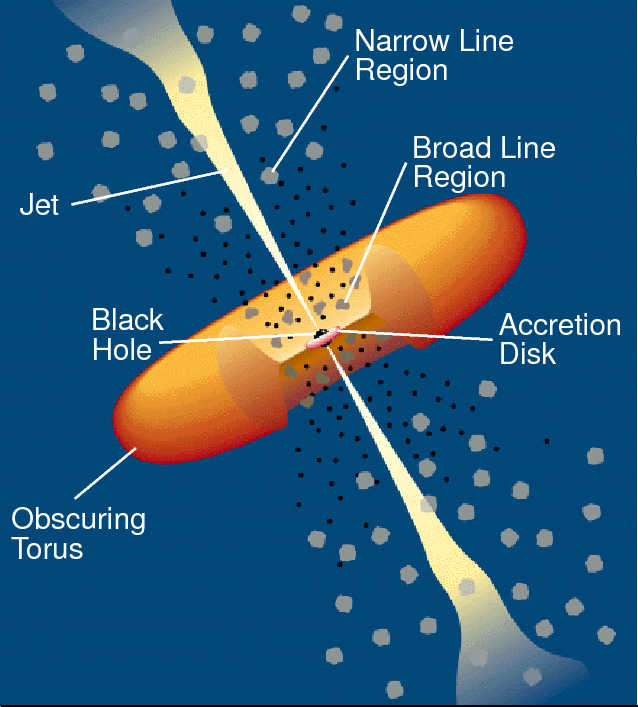
\includegraphics[width=0.5\textwidth]{figures/chapter05/urry_model}
  \caption{Illustration of the physical structure of an AGN in a simple orientation-based unification model. From \citet{urry95}.}
  \label{fig:agnmodel}
\end{figure}

AGNs are divided into numerous classes and sub-classes based on their observational properties. 
AGN unification models \citep{antonucci93,urry95} attempt to explain the diversity in their observational properties using as few physical parameters as possible. 
In many unification models the optical and radio luminosities are considered to be intrinsic parameters. Variations in the radio luminosity explains the difference between the $15-20\%$ of AGN which are {\it radio-loud} (i.e. have radio to optical flux ratios $\gtrsim$ 10) and the remainder which are {\it radio-quiet}. 
The optical luminosity explains, for example, the difference between low-luminosity {\it Seyfert Galaxies} and high-luminosity {\it quasars}\footnote{The term `quasar' is sometimes reserved for radio-loud objects and `quasi-stellar object', or `QSO', for radio-quiet objects. Here, `quasar' is used to refer to all luminous AGN.}.
In a typical quasar the optical emission may be brighter than the combined emission from all of the stars in the host galaxy by a factor of 100 or more. 
The large brightness contrast between the nucleus and the host galaxy makes the host galaxy difficult to detect, and the quasar is observed as an unresolved stellar-like object\footnote{The name `quasar' is shortened from `quasi-stellar radio source', since quasars were originally discovered as optical point-source counterparts to a newly discovered population of radio sources.}.   

Unification models attempt to explain all further observational differences as being apparent differences due to {\it orientation} effects. 
The basic physical structure of an AGN in this model is illustrated in Figure \ref{fig:agnmodel}. 
Material is pulled towards the SMBH at the centre and sheds angular momentum through viscous and turbulent processes in an accretion disk, which radiates primarily at ultraviolet (UV) to soft-X-ray wavelengths. 
Strong optical and UV emission lines are produced in photo-ionised gas clouds moving rapidly in close proximity to the SMBH. 
The doppler-broadened emission line widths imply gas cloud velocities of thousands of km s$^{-1}$ in this {\it broad-emission line}. 
Further out are dusty, molecular clouds, the geometry of which is often modelled as a torus co-planar with the accretion disk. 
Along some lines of sight from the observer to the accretion disk / broad line region the dusty torus obscures the UV/optical radiation. 
In this case, an observer would see a weak UV/optical continua and no broad emission lines and classify the AGN as being {\it Type II}. 
On the other hand, if the line of sight is unobscured by the dusty torus then a broad emission line component would be observable in the spectrum and the AGN would be classified as being {\it Type I}. 
Further away from the central black hole and beyond the dusty torus are slower moving clouds of gas which are photo-ionised by the continuum emission from the accretion disk and produce forbidden emission lines of narrower widths (typically hundreds of km s$^{-1}$). 
Outflows of energetic particles occur along the poles of the accretion disk and form collimated radio-emitting jets and in some cases giant radio-emitting lobes. 
A strong, relativistically beamed component with large variations in brightness on very short timescales (e.g. ${\Delta}m \gtrsim 0.1$ and $\Delta t \lesssim 1$ day) is observed and a source with these properties is classified as a {\it blazar}. 

While an orientation-based unification scheme such as this is somewhat successful at explaining many of the observational properties of AGNs, other factors such as the host galaxy morphology and gas/dust content may also be important \citep{peterson95}. 
It is also doubtful whether the geometry of the dusty torus is the same in all AGNs, and the fraction of obscured quasars has been shown to decrease with increasing nuclear luminosity \citep{lawrence91}. 
As we will now discuss, quasars might play an important role in a broader cosmological context, affecting the formation and evolution of the galaxies, groups, and clusters in which they reside. 
In this scenario of galaxy/quasar co-evolution the quasar is expected to transition from a highly active obscured phase to an unobscured phase as it clears out the dust surrounding it. 
If this picture is true then we should expect to find variations in the observational properties of the quasar and host galaxy as the system transitions through the different stages of its evolution.  

\section{The Torus}

Elitzur \& Shlosman (2006): 

Recent high-resolution IR observations indicate that the torus size might be no more than a few parsecs (Elitzur 2005 and references therein); in particular, VLTI observations of NGC 1068 show that the FWHM size of the 12 mm emission is only 4 pc (Jaffe et al. 2004). The compact sizes place the torus inside the region where the SBH gravity dominates over the galactic bulge.

Two approaches have been taken for the torus dynamic origin. A hydrostatic scenario depicts the torus as a doughnut-like structure populated by molecular clouds accreted from the galaxy (Krolik \& Begelman 1988). However, the origin of vertical mo tions capable of sustaining the clouds in a hydrostatic structure with H$\sim$R was recognized from the start as problematic and has eluded solution thus far (e.g., Davies et al. 2006). The other
scenario, based on the seminal work by Blandford \& Payne (1982), involves the outflow of clouds embedded in a hydromagnetic disk wind (Emmering et al. 1992, hereafter EBS92; Konigl \& Kartje 1994; Kartje \& Konigl 1996; Bottorff et al. 1997, 2000; Kartje at al. 1999; Everett 2005). In this approach the torus is merely a region in the wind that happens to provide the required toroidal obscuration; i.e., it is that region wherein the clouds are dusty and optically thick.



\section{Evolutionary Models}

A number of observations link the growth and evolution of quasars to the growth and evolution of galaxies. These include the following: 

\begin{enumerate}
\item SMBHs appear to be a ubiquitous feature at the centres of all massive galaxies \citep[e.g.][]{kormendy13}. 
\item SMBH masses are proportional to the mass/velocity dispersion of their host spheroid \citep[the $M-\sigma$ relation;][]{ferrarese00,gebhardt00}.
\item The cosmological evolution of the star formation rate and the quasar luminosity function are very similar \citep[e.g.][]{wall05}.
\item Cosmological simulations of galaxy formation and evolution require feedback from SMBH growth in order to reproduce the galaxy luminosity function \citep{kauffmann00}.
\end{enumerate}

These observations suggest that all galaxies may have gone through a `quasar phase' during which the SMBH accretes most of its mass and the stellar-bulge forms most of its stars. 
This evolutionary phase could be triggered by a major merger or by instabilities in the galactic disc or bulge. 
In a galaxy merger large amounts of gas can shed sufficient angular momentum to settle into dense clouds and form stars or be funnelled to the centre of the galaxy to grow the existing SMBH. 
The large amounts of gas and dust funnelled inward to the galactic nucleus is predicted to obscure the quasar until the dust is cleared out either by quasar-driven or stellar-driven processes. 
An un-obscured quasar then emerges, and is active until all of the available material has been accreted \citep{hopkins06a, narayanan10}. 
The feedback processes involved are also thought to be responsible for shutting down star formation in the galactic bulge \citep{silk98} and establishing the $M-\sigma$ relation. 

Such scenarios have been invoked to explain the presence of buried AGN seen in ultra-luminous infra-red galaxies \citep[ULIRGs;][]{sanders88}, a high fraction of which also show evidence of merging and interaction. 
However, the full picture is likely to be more complicated. Although there is evidence that mergers dominate at high luminosities \citep{treister12}, stochastic accretion may be more important at low luminosities \citep[e.g.][]{hopkins06b}. 

Luminous unreddened quasars show few signs of interaction \citep[e.g.][]{dunlop03} which, if the quasar-galaxy co-evolution model is true, suggests that indications of an interaction disappear during a transitional phase. Quasars in this transitional phase would be highly reddened, as the dust enshrouding the nucleus will not have been fully cleared, but not completely obscured. 
A population of quasars with these properties may therefore represent a link between ULIRGs and unobscured quasars. 

\section{Interesting Sub-Populations}

\subsection{Red and Reddened Quasars}

Magnitude limited optical surveys of quasars are biased against selecting red and reddened quasars. 
\citet{richards03} studied a large sample of optically selected Sloan Digital Sky Survey \citep[SDSS;][]{york00} quasars and showed the mean reddening to be $E(B-V) = 0.03$ at the redshift of the quasar. 
They estimated that $\sim 15\%$ of the population was missing from the survey due to dust extinction. 
The missing fraction, and it's dependence on luminosity and redshift, could help to determine whether the reddened population is best explained in the context of orientation-based unification models with non-spherical geometry or as an evolutionary stage in a quasars lifetime.   

Populations of heavily dust-reddened quasars have been identified using radio surveys \citep[e.g.][]{glikman12}, by using the `$K$-band excess' in the spectra of quasars relative to stars \citep{maddox12}, and using near-IR colour selection \citep{banerji12,banerji13}. 
Recently, \citet{ross14} identified a small sample of very red SDSS quasars based on their extreme IR to optical luminosity ratios. 
It is yet to be determined whether these extreme objects are simply the tail of a population dominated by less reddened quasars, or whether the distribution is bi-modal with reddening. 
A population of quasars with intermediate amounts of dust reddening ($0.1 \lesssim {\rm E(B-V)} \lesssim 0.5$) would help to address this question. 

\subsection{Broad Absorption Line Quasars}

{\it Broad absorption line quasars} (BALQSOs) are a sub-population of quasars exhibiting blue-shifted absorption troughs broader than 2000kms$^{-1}$ \citep{weymann91} which are unambiguously associated with AGN-driven out-flowing gas. 
As well as showing high rates of mergers, an anomalously large fraction of heavily reddened objects exhibit broad blue-shifted absorption troughs in their spectra \citep{urrutia09, glikman12}. 
This observation suggests that the BAL phenomenon may be related to a `blow-out' phase of a quasars lifetime as it transitions from a dusty, obscured objected to a luminous blue quasar, at the same time quenching star formation. Since outflows are believed to be fundamental to AGN feedback, a better understanding of their properties could shed light on the outflow phenomenon. 
Alternatively, whether a quasar is observed to have broad absorption lines could depend only on the orientation of the observer in relation to an intrinsically anisotropic system.

\subsection{Hot-Dust-Poor Quasars}

The near-IR emission from AGN is generally explained by thermal emission from dust grains at the edge of the dusty torus closest to the accretion disk. 
The dust is heated to its sublimation temperature \citep[1300-2000K][]{barvainis92} by emission from the accretion disc. However, \citet{hao10} reported that 6\% (at $z \lesssim 2$) to 20\% (at $2 \lesssim z \lesssim 3.5$) of the quasars in the X-ray selected XMM-COSMOS Type 1 AGN sample \citep{brusa10} have an unusually small amount of hot dust emission, despite having normal accretion disc spectra. 
They infer a torus covering factor of  $\sim$2\% to 30\% for these `hot dust poor' (HDP) quasars, well below the $\sim$75\% predicted by unified models \citep[e.g.][]{krolik88}. 
\citet{hao11} found that HDP quasars were just as common in the \citet{richards06} Spitzer/SDSS sample ($8.7\% \pm 2.2\%$) and the \citet{elvis94} Palomar-Green-quasar-dominated sample ($9.5\% \pm 5.0\%$). 
Either the hot dust is destroyed (dynamically or by radiation), or the dust is not centred on the SMBH, which could happen during a major merger \citep[e.g.][]{blecha11}. 
Alternatively, misaligned accretion disks, which will result from discrete isotropic accretion events \citep{volonteri07}, will lead to a wider range of covering factors \citep{lawrence10}. 

At higher redshifts, \citet{jiang10} found two HDP quasars in a sample of 21 at $z\sim6$. 
They find that at $z\sim6$ the hot dust abundance is roughly proportional to the black hole mass, indicating that the two grow at about the same rate. 
The two HDP quasars also have the smallest SMBH masses, and may be too young to have formed a significant amount of hot dust.

\subsection{Type II Quasars}

As well as lacking a broad-line spectral component, Type II AGN tend to have high IR to optical light ratios, hard X-ray spectra, and be strongly polarised, consistent with dusty torus based unification schemes. 
The detection of unobscured continuum emission that is scattered and polarised by dust above the torus has confirmed the orientation-based unification of Type I and Type II Seyfert Galaxies. 
Their higher luminosity analogues, Type II quasars, have been much more difficult to detect and study. 
It is possible that the orientation-based Type I/II unification scheme may break down at high-luminosities, and that instead all quasars could pass through a Type II phase before the obscuring dust is cleared out by the quasar-driven outflows and a Type I quasar emerges.  

\section{Spectral Energy Distributions}
\label{sec:sed}

\begin{figure}
  \centering
  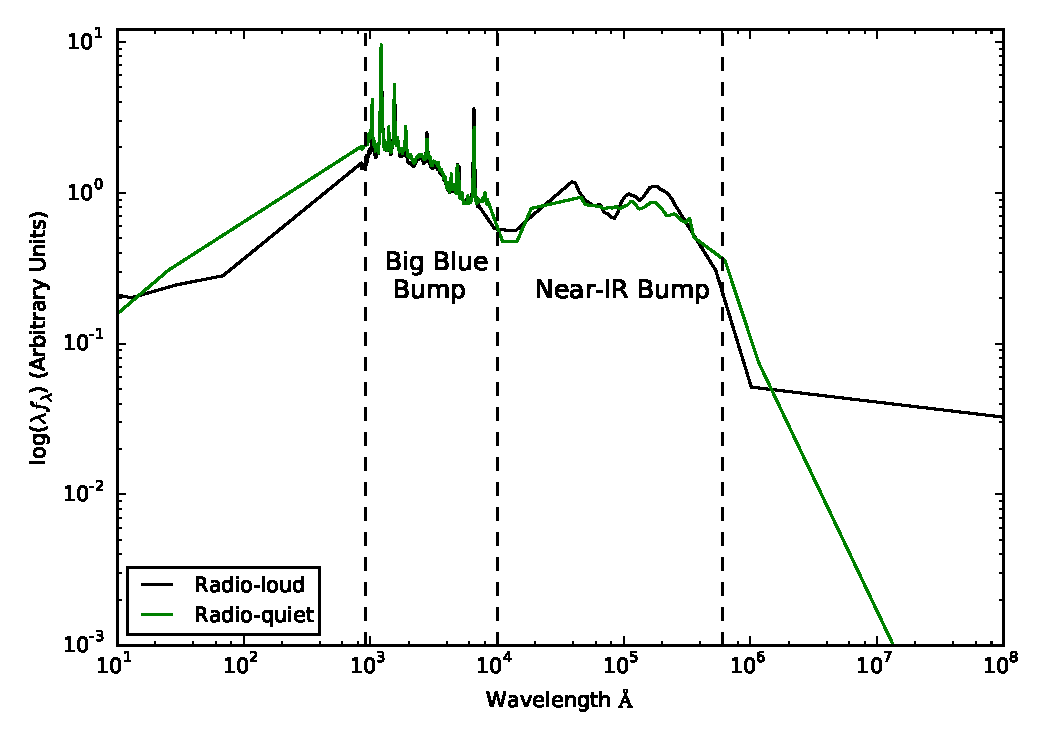
\includegraphics[width=\textwidth]{figures/chapter01/shangsed.pdf}
  \caption{Median SEDs for radio-loud and radio-quiet quasars from \citet{shang11}.}
  \label{fig:seyfert_sed}
\end{figure}

AGNs emit strongly over many decades in frequency of the electromagnetic spectrum and the energy emitted as a function of frequency is described by a {\it spectral energy distribution} (SED). 
As we will describe below, the broad features in the SED originate from processes which occur in different regions of the AGN. 
In the preceding sections, we have described how some interesting sub-populations of AGNs might relate to the broader population in the context of orientation-based unification schemes and evolutionary schemes. 
Comparing SEDs of different sub-populations can help to shed light on these relationships and the physical processes which drive them. 
Possible correlations between the SED shape and luminosity, redshift, and other properties of the AGN such as black hole mass and Eddington ratio can also constrain models of AGN structure and evolution. 

Since the physical processes involved are generally understood only qualitatively, almost all AGN SED templates are empirical. 
The empirical template of \citet{elvis94}, constructed using photometric observations from the radio to the hard X-rays of 29 radio-quiet and 18 radio-loud Type I quasars, is still the most commonly cited, despite many additions and updates \citep[e.g.][]{polletta00, kuraszkiewicz03, risaliti04, richards06,  polletta07, lusso10, shang11, marchese12, trichas12}. 
In Figure \ref{fig:seyfert_sed} we show the median spectrum from the radio-loud and radio-quiet samples of Shang et al. (2011). 
Short-ward of the radio region, the radio-loud and radio-quiet spectra are almost indistinguishable. 

A large amount of energy is emitted in the UV/optical region short-ward of $\sim4000$\AA: the {\it Big Blue Bump}. In the X-ray region, the {\it soft X-ray excess} may be the high-energy end of this feature. 
The Big Blue Bump is generally attributed to thermal emission from the accretion disk. 
In Type II AGNs, the continuum emission from the accretion disk is obscured, and so the Big Blue Bump in the SED of a Type II AGN would be less prominent than is seen in Figure \ref{fig:seyfert_sed}. 

The feature at wavelengths long-ward of $\sim1\mu$m is the {\it IR Bump}, and is generally attributed  to thermal emission from dust at a wide range of temperatures ($\sim50 - 1000$ K). 
The amount, geometry, ionisation and optical depth of absorbing dust and gas and its inclination determines the shape of the IR Bump and the absorption of the optical/UV continua. 
The relative strengths of the IR Bump and the Big Blue Bump are generally comparable, although they do vary from object to object. 
In particular, for the HDP objects we described above the IR Bump appears to be missing entirely. 
The minimum between the two peaks is at $\sim1\mu$m, which reflects the sublimation of dust at T $\gtrsim 2000$ K \citep{sanders89}.

Emission in the hard X-ray region of the spectrum is believed to be due to Compton up-scattering of accretion disk photons by hot electrons forming a corona in the vicinity of the disk \citep[e.g.][]{sunyaev80}. 
The radio emission, which originates from synchrotron emission in relativistic jets, contributes very little to the total energy output.
However, the mechanical energy provided by the jets is an important component of AGN feedback models \citep[e.g.][]{fabian12}. 

Many parameters might be expected to affect the shape of the AGN SED (e.g. the black hole mass, the accretion rate, the physical properties of the accretion disk, the properties of the absorbing dust) and many of these properties might be expected to change as the quasar evolves (e.g. as dust is expelled from the nuclear regions). Given this, it is perhaps surprising that many authors have found no significant dependence of the mean SED on properties such as redshift, bolometric luminosity, SMBH mass, or accretion rate \citep[e.g.][]{elvis12,hao13} and that quasars up to redshift 7 have been shown to have similar UV spectra to low redshift quasars \citep[e.g.][]{mortlock11}.

Throughout this thesis we adopt a $\Lambda$CDM cosmology with $h_0=0.71$, $\Omega_M=0.27$, and $\Omega_\Lambda=0.73$. 
All wavelengths and equivalent width measurements are given in the quasar rest-frame, and all emission line wavelengths are given as measured in vacuum.

Everett et al. (2005): 

A variety of observational signatures point to the importance of outflowing gas within many types of active galactic nuclei (AGNs). Blueshifted absorption features (in broad absorption line quasars, or BALQSOs; see, e.g., Weymann et al. 1991) are seen in approximately 15\% (Reichard et al. 2003) of radio-quiet quasars, with velocities up to 0.1c. In addition, radio-loud quasars display relativistic, collimated outflows. 
There has also been observational evidence that suggests the mass outflow rate in AGNs is nearly equal to the mass inflow rate (see, e.g., Crenshaw et al. 2003; Chartas et al. 2003).
